%%%%%%%%%%%%%%%%%%%%%%%%%%%%%%%%%%%%%%%%%%%%%%%%%%%%%%%%%%%%%%%%%%%%%%%% 
%%%%%%%%%%%%%%%%%%%%%%%%%%%%%%%%%%%%%%%%%%%%%%%%%%%%%%%%%%%%%%%%%%%%%%%% 
\begin{frame}[fragile=singleslide]
  \frametitle{Hands-On 3 : Mandelbrot set}

  \begin{itemize}
  \item \textcolor{darkgreen}{\textbf{Illustrate Functor class + 1D \texttt{Kokkos::View} + linearized index}}
  \item the original \textcolor{red}{serial code} use 1D \texttt{std::vector<unsigned char>} data with linearized index, i.e. $index = i + Nx * j$
  %\item Read carefully the original \texttt{serial/main.cpp} (notice the use of global variables)
  \item See \textcolor{red}{serial code} from \texttt{code/exercises/mandelbrot\_kokkos/serial} (also read \textcolor{red}{\texttt{main.cpp}})
    {\small
      \begin{minted}{c++}
        for(int index=0; index<WIDTH*HEIGHT; ++index) {
          int i,j;
          index2coord(index,i,j,WIDTH,HEIGHT);
          image[index]=mandelbrot(i,j);
        }
      \end{minted}
    }
  \end{itemize}

  \begin{center}
    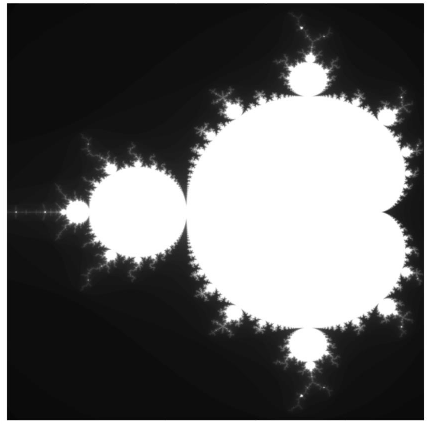
\includegraphics[width=4cm]{images/mandelbrot}
  \end{center}
  
\end{frame}

%%%%%%%%%%%%%%%%%%%%%%%%%%%%%%%%%%%%%%%%%%%%%%%%%%%%%%%%%%%%%%%%%%%%%%%% 
%%%%%%%%%%%%%%%%%%%%%%%%%%%%%%%%%%%%%%%%%%%%%%%%%%%%%%%%%%%%%%%%%%%%%%%% 
\begin{frame}[fragile=singleslide]
  \frametitle{Hands-On 3 : Mandelbrot set}

  {\Large \textcolor{darkgreen}{\textbf{Proposed activity:}}\\ \textbf{refactor this computing loop into a C++ Kokkos functor class}}
  \begin{itemize}
  \item See \textcolor{blue}{kokkos basic version} from \texttt{code/exercises/mandelbrot\_kokkos/kokkos\_basic} (already a bit refactored to ease the job)
  \end{itemize}
  %
  \begin{enumerate}
  \item we added a file \textcolor{blue}{\texttt{kokkos\_shared.h}}: \texttt{std::vector} replaced by a \texttt{Kokkos::View}
  \item \textcolor{orange}{\textbf{TODO:}} fill TODOs in \texttt{mandelbrot.h} containing the definition of the c++ mandelbrot kokkos functor.\\
    \textbf{Notice:} the global constants have disappeared, they are now part of the functor context.
  \item \textcolor{orange}{\textbf{TODO:}} refactor \texttt{main.cpp} (change the TODO)
    \begin{itemize}
    \item Modify data allocation (from \texttt{std::vector} to \texttt{Kokkos::View}); we have now arrays: \texttt{image} and \texttt{imageHost} (mirror)
    \item Copy back results from device to host.
    \end{itemize}
  \end{enumerate}
  
\end{frame}

%%%%%%%%%%%%%%%%%%%%%%%%%%%%%%%%%%%%%%%%%%%%%%%%%%%%%%%%%%%%%%%%%%%%%%%% 
%%%%%%%%%%%%%%%%%%%%%%%%%%%%%%%%%%%%%%%%%%%%%%%%%%%%%%%%%%%%%%%%%%%%%%%% 
\begin{frame}[fragile=singleslide]
  \frametitle{Hands-On 3 : Mandelbrot set}

  \begin{itemize}
  \item Build the \texttt{kokkos\_basic} version
  \item OpenMP
    \begin{itemize}
    \item \texttt{module use /pwrwork/workshops/patc-201701/kokkos/modulefiles}
    \item \texttt{module load kokkos/openmp_gnu485_dev}
    \end{itemize}
  \item Cuda
    \begin{itemize}
    \item \texttt{module use ...}
    \item \texttt{module load cuda/8.0 kokkos/cuda80_gnu485_dev_k80}
    \end{itemize}
  \item Compare performance for a large Mandelbrot set $8192\times 8192$
  \end{itemize}

\end{frame}
  
%%%%%%%%%%%%%%%%%%%%%%%%%%%%%%%%%%%%%%%%%%%%%%%%%%%%%%%%%%%%%%%%%%%%%%%% 
%%%%%%%%%%%%%%%%%%%%%%%%%%%%%%%%%%%%%%%%%%%%%%%%%%%%%%%%%%%%%%%%%%%%%%%% 
\begin{frame}[fragile=singleslide]
  \frametitle{Hands-On 3 : Mandelbrot set}

  \begin{itemize}
  \item Understand what is missing to match pipelined version see
    \myurl{http://on-demand.gputechconf.com/gtc/2015/webinar/openacc-course/advanced-openacc-techniques.pdf}
  \item See explanations given during training
  \end{itemize}

\end{frame}